% !TEX encoding = UTF-8 Unicode
\label{sec:expre}
Além do que foi solicitado como obrigatório para essa entrega, 
pensamos ser importante definir a forma como fizemos a implementação do 
cálculo de expressões para a geração de código de saída.

Como o professor Ricardo Rocha nos explicou, a MVN não tem uma implementação
real de pilha, porém consegue simular a existência de uma pilha com o uso de
indirecionamentos que definem cada uma das operações da pilha, como \emph{push}
e \emph{pop}. Baseado nesse conceito de código alinhavado, definimos diversas
funções auxiliares que realizam operações simples de forma independente. Essas
funções nos permitiram realizar o cálculo de expressões de maneira mais clara e
com menos erros.

Para explicar de forma mais detalhada o processo utilizado para calcular as
expressões, vamos supor que lemos uma expressão \verb=1 + 2 * 3=. A gramática
que já implementamos nas etapas anteriores cria uma árvore que já considera a
ordem de prioridade das operações, fazendo com que a multiplicação ocorra antes
da soma. Para esse caso, o código de máquina deve primeiro empilhar o 1, em
seguida o 2 e depois o 3. Ao notar que uma operação de multiplicação foi
finalizada, ele retira da pilha dois operandos, no caso o 2 e o 3, realizando a
multiplicação e retornando a pilha o resultado da operação, no caso 6. Em
seguida, é efetuada a operação de soma com os dois operandos que estão na
pilha, o 1 e o 6, adicionando novamente o resultado, 7, na pilha.

\begin{figure}[htbp]
    \centering
    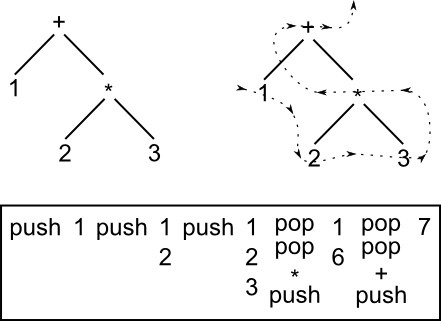
\includegraphics[width=.6\textwidth]{./img/arith.png}
    \caption{Árvore da expressão e operações resultantes na pilha.}
    \label{figure:example}
\end{figure}

O mesmo tipo de lógica foi implementado também para operadores booleanos e
permite a geração de código de forma mais simples, visto que já desenvolvemos
funções auxiliares para essas operações.

Apresentamos abaixo as operações principais da pilha aritmética. Todas as
outras operações da pilha se encontram no arquivo \verb!std.asm! no final do arquivo.


\begin{lstlisting}[frame=single,numbers=left,breaklines=true]
;--------------------------PUSH_ARITH------------------------------
PUSH_ARITH      JP /000
                MM TMP_1
                LD ARIT_PTR_STACK 
                +  TWO
                MM ARIT_PTR_STACK
                +  MOVE_CONST
                MM OP_PUSH_ARITH
                LD TMP_1
OP_PUSH_ARITH   JP /000 
                RS PUSH_ARITH 
;--------------------------POP_ARITH-------------------------------
POP_ARITH       JP /000 
                LD ARIT_PTR_STACK 
                -  TWO
                MM ARIT_PTR_STACK 
                +  TWO 
                +  LOAD_CONST 
                MM OP_POP_ARITH
OP_POP_ARITH    JP /000
                RS POP_ARITH 
;--------------------------SUM_ARITH-------------------------------
SUM_ARITH       JP /000 
                SC POP_ARITH
                MM TMP_2 
                SC POP_ARITH
                +  TMP_2 
                SC PUSH_ARITH
                RS SUM_ARITH 
;--------------------------MUL_ARITH-------------------------------
MUL_ARITH       JP /000 
                SC POP_ARITH
                MM TMP_2 
                SC POP_ARITH 
                *  TMP_2 
                SC PUSH_ARITH
                RS MUL_ARITH 
\end{lstlisting}
